After all of the jargon, we get into the good stuff. This section focuses on developing the framework we'll use later on in order to do some risk management.

\subsection*{Value and Loss}
We denote the value of a portfolio as $V$ (mathematically, a stochastic process) where at each time $t$ the value of the portfolio is defined as $V_t = V(t)$. Then,
each random variable $V(t)$ is observable at time $t$.

\begin{definition}
    For a given risk horizon $\Delta$, we define the loss of a portfolio $V$ over the period $ \left[ t, t + \Delta \right] $ as
    $$\mathcal{L}(t, t + \Delta) = - (V_{t + \Delta} - V_t)$$
    this is observable at time $t + \Delta$ but is `random' at $t$. This distribution is called the \textit{loss distribution}.
\end{definition}

\vspace{0.2cm}

A large positive value of $L$ indicates that the portfolio suffered a large decrease in value over $\left[ t, t + \Delta \right]$. We also define the \textbf{negative} of the loss function,
called the Profit-and-loss distribution i.e. $PnL(t, t + \Delta) = - \mathcal{L}(t, t + \Delta)$.

\begin{figure}[htbp]
\centerline{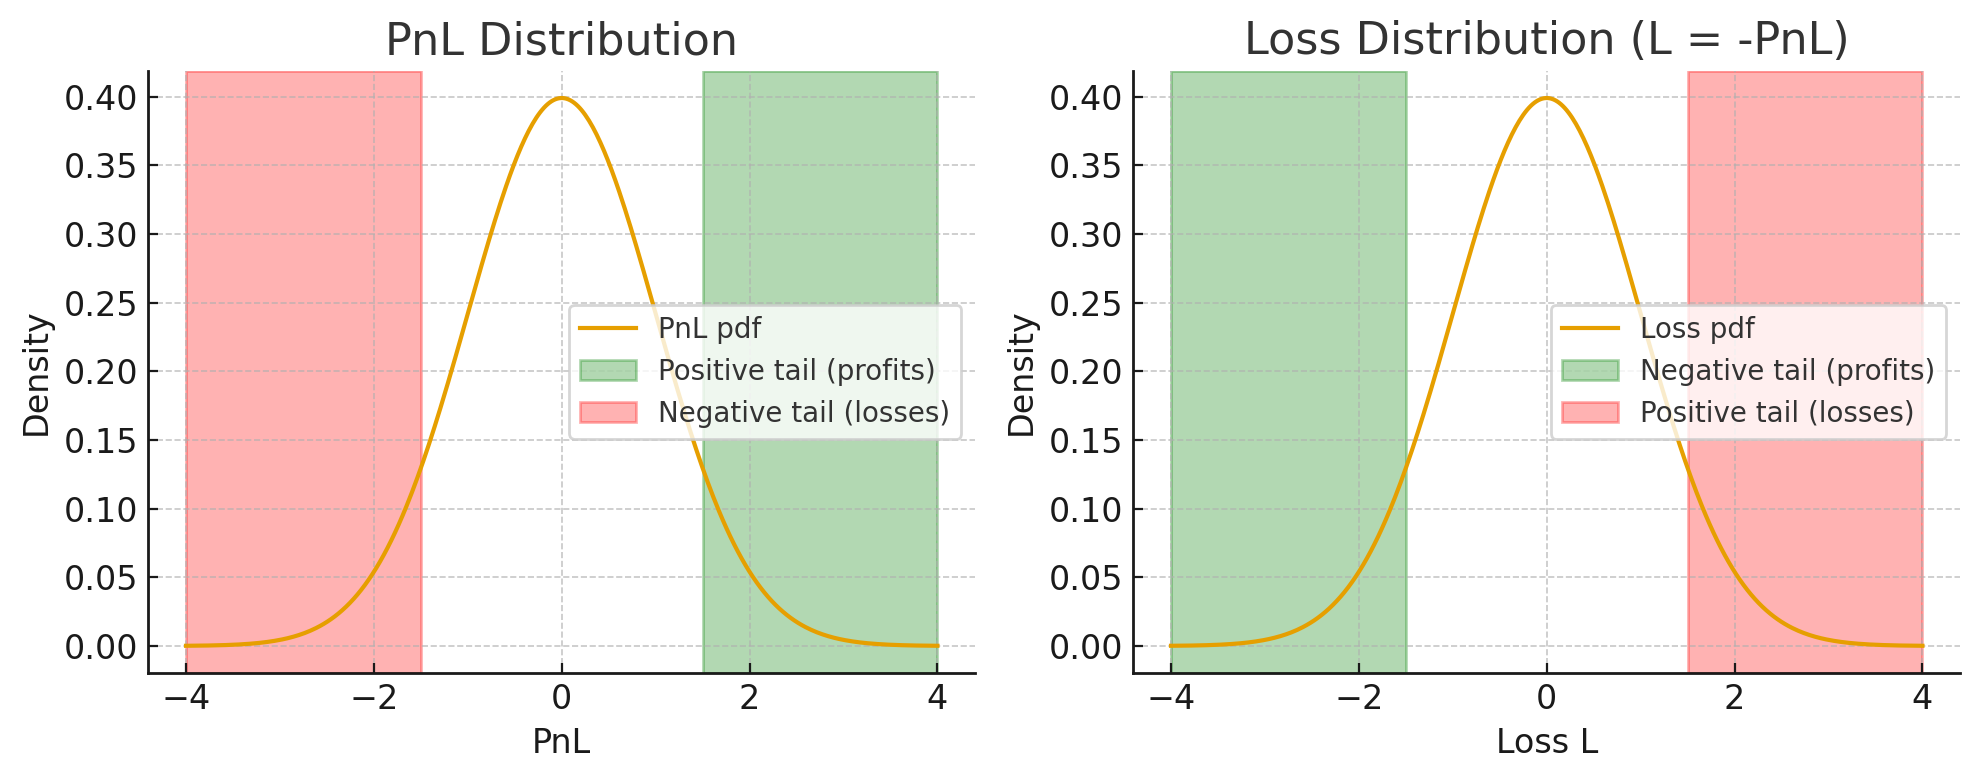
\includegraphics[scale=0.5]{figures/pnl_v_l_distributions.png}}
\caption{PnL v. Loss distribution}
\label{lossvpnl}
\end{figure}

\begin{remark}
    Much of risk management is focused on the negative tail of the PnL distribution, which is equivalent to the possitive tail of the loss distriution. 
\end{remark}

Sometimes, we may not have a full understanding (or any at all) of $\mathcal{L}$. It is also important to know that we may sometimes model $V$ as a function of
several risk factors. This suggests the following notation:

\begin{itemize}
    \item $V_t = f(t, Z_t)$: value of portfolio as function of underlying risk factors.
    \item $Z_t = (Z_{1,t}, \ldots, Z_{d, t})$: underlying risk factors; often representing stock value, intrest rate, etc.
    \item $f: \mathbb{R} \times \mathbb{R}^d \rightarrow \mathbb{R}$: measurable function.
    \item for $V_t$ to be observable at time $t$, we must have $Z_{k,t}$ observable at $t \text{  } \forall k$
\end{itemize}

The choice for each $Z_k$ and $f$ is a modeling issue.

\begin{definition}
    We define the vector of risk factor changes as $X_{t + \Delta} = Z_{t + \Delta} - Z_t$ and so, we may redefine the loss distribution as
    $$\mathcal{L}(t, t + \Delta) = - \left( V_{t + \Delta} - V_t \right) = - \left( f(t + \Delta, Z_{t + \Delta}) - f(t, Z_t) \right) $$
    $$\Rightarrow \mathcal{L} = - \left( f(t + \Delta, X_{t + \Delta} + Z_t) - f(t, Z_t) \right)$$
\end{definition}

The loss distribution is fully determined by the distribution of $X_{t + \Delta}$ and the function $f$. If $f$ is differentiable, we sometimes consider a first-order taylor approximation of the loss as
$$\mathcal{L}^{\delta}(t, t + \Delta) = - \left( \partial_t f(t, Z_t) \Delta + \sum_{i=1}^{d} \partial_{Z_i} f(t, Z_i)X_{i, t + \Delta} \right)$$

\begin{remark}
    Note that this aproximation is good whenever $\Delta$ is small enough. This may be observed in figure \ref{firstorderaprox}.
\end{remark}

\begin{figure}[htbp]
\centerline{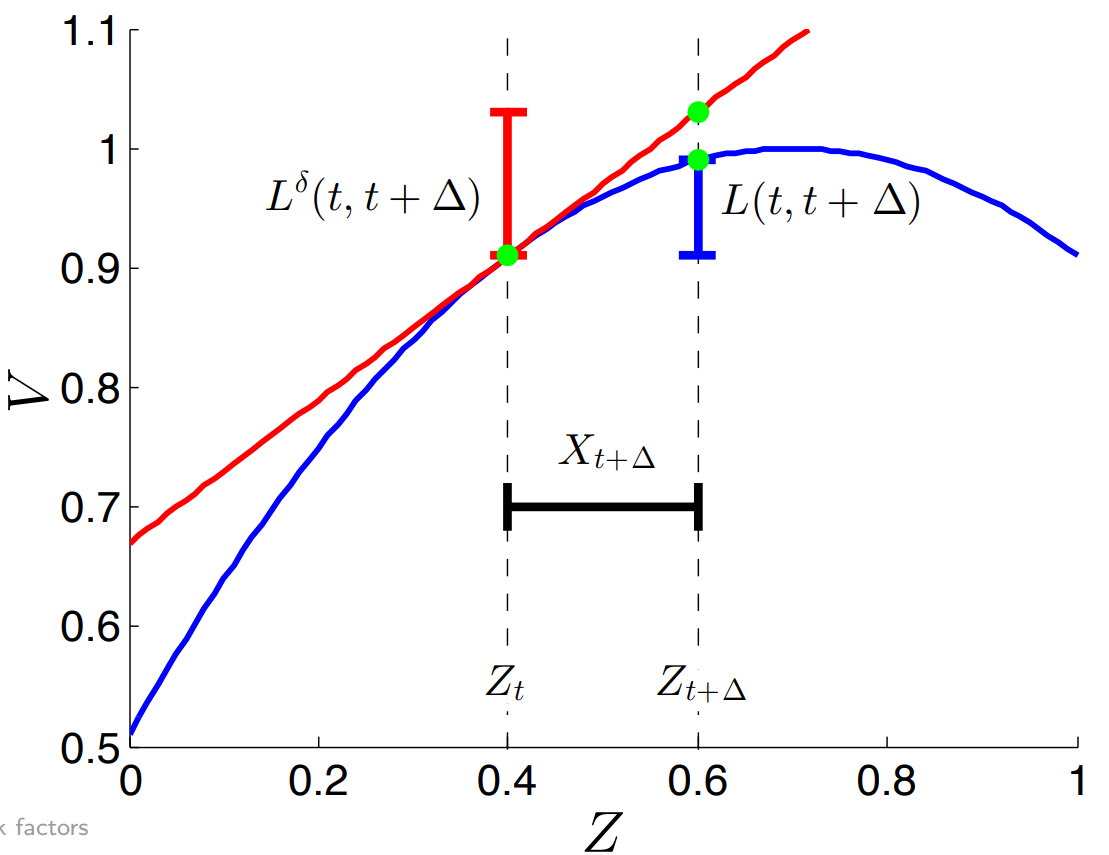
\includegraphics[scale=0.2]{figures/linear_approx_lossdistribution.png}}
\caption{First order Taylor aproximation of $\mathcal{L}$}
\label{firstorderaprox}
\end{figure}